\chapter{Mathematical Formulation}
\label{chapter-mathematical-formulation}
 
This chapter describes the mathematical formulation of the single-phase flow equation, which constitutes the basic framework for the simulator developed. 
%
The next chapters will show how this equation has been discretized and linearized for allowing its solution by numerical methods.
%
Next, the well modeling process will be shown in a succeeding chapter, along with its attachment to the single-phase flow equation.
%
Finally, a later chapter will show how the resulting system of equations will be linearized and solved for the boundary conditions of the problem.
\begin{figure}[H]
 	\centering
 	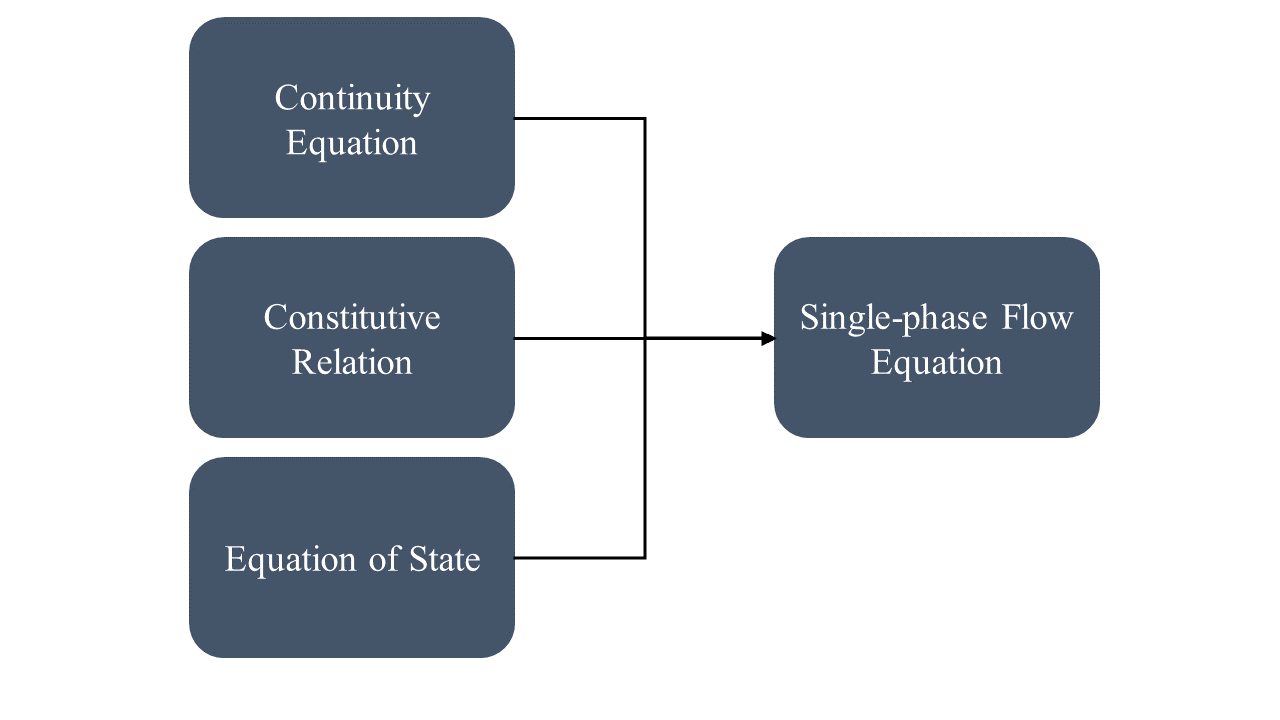
\includegraphics[width=0.8\textwidth]{figure-origin-of-the-single-phase-flow-equation.png}\\
 	\caption{Diagram illustrating the development of the single-phase flow equation.}
 	\label{figure-origin-of-the-single-phase-flow-equation}
\end{figure}

According to \cite{Ertekin2001}, the single-phase flow in porous media can be modeled by utilizing three fundamental equations: the equation of continuity (or mass conservation) which relates the mass quantity of the incoming and outgoing components with the accumulated mass in a given control volume; a constitutive relation, which describes the fluid momentum in the control volume; and an equation of state, relating the specific mass of the fluid in the function of its pressure, temperature, and composition.
%
The following sections show the development of those three equations: the continuity equation, constitutive relation, and equation of state. Later, a posterior section shows how those three equations will be assembled into the single-phase flow equation.
  
\section{Continuity Equation}

The equation of continuity can be developed by utilizing the continuum assumption.
%
This is the assumption that on a macroscopic scale, certain proprieties in a fluid such as density, temperature, pressure, and velocity can be defined at infinitesimal volume elements.
%
Those elements are representative sampling volumes of the propriety, so it is possible to neglect the microscopic discontinuities.
%
Thus, it is possible to assume that those variables vary continuously from one control volume to another.
%
According to \cite{Fox2008}, the continuum assumption is one of the bases of classical fluid mechanics.
%
\begin{figure}[H]
	\centering
	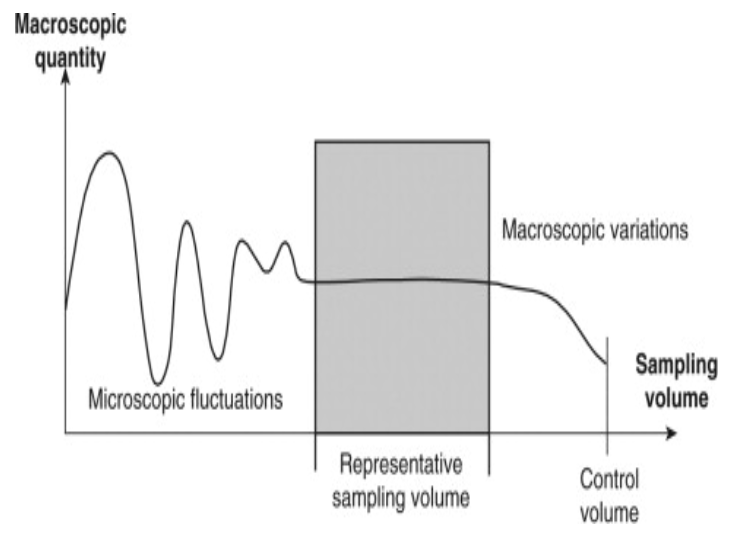
\includegraphics[width=0.7\textwidth]{figure-continuum-assumption.png}
	\caption{The variation of a given macroscopic propriety in different levels of scale. Source: \cite{Kandlikar2014}.}
	\label{figure-continuum-assumption}
\end{figure}
\noindent
%
With this assumption, the reservoir proprieties (e.g., porosity and permeability) can be described in terms of the average values in a control volume.
%
Figure \ref{figure-control-volume} represents a control volume in a Cartesian coordinate system.
%
	\begin{figure}[H]
	\centering
	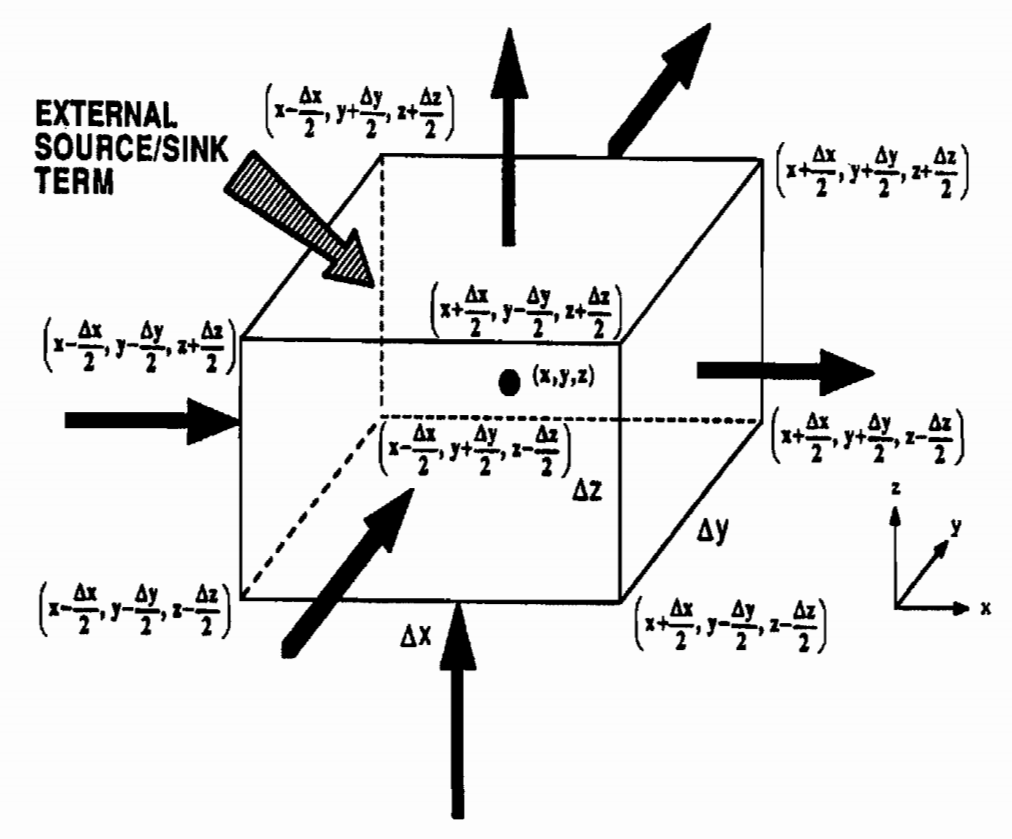
\includegraphics[width=0.6\textwidth]{figure-control-volume.png}\\
	\caption{Example of a control volume in a Cartesian coordinate system. Source: \cite{Ertekin2001}.}
	\label{figure-control-volume}
	\end{figure}

Mass conservation principle for classical fluid dynamics states that mass can neither be created nor destroyed within a closed system. If the inflow mass flow rate is different from the outflow mass flow rate for a closed system, then necessarily there should be variations in volume or density within that system. Mathematically:
%
\nomenclature[R]{$m$}{Mass}
\nomenclature[R]{$m_i$}{Incoming mass in a control volume}
\nomenclature[R]{$m_o$}{Outgoing mass in a control volume}
\nomenclature[R]{$m_s$}{Mass that enters or leaves a control volume trough inside boundaries (wells)}
\nomenclature[R]{$m_a$}{Mass that accumulates inside a control volume}
%
\begin{align}
	\label{equation-mass-conservation}
	(m_i-m_o)+m_s=m_a ,
\end{align}
%
in which $m_i$ and $m_o$ are, respectively, the incoming and outgoing mass in the control volume faces, $m_a$ is the accumulated mass inside it and $m_s$ is the source term, which represents the mass that is added or removed in the control volume but not passes through the external boundaries (a source term typically represents the well in the case of a reservoir simulator).
%
A quantity of mass $m$ can also be described by:
%
\nomenclature[R]{$w$}{Mass flow rate}
\nomenclature[R]{$t$}{Time}
%
\begin{align}
	\label{equation-quantity-of-mass}
	m = w \Delta t ,
\end{align}
%
where $w$ is the average mass flow rate in a time interval of $\Delta t$. The mass flow rate can also be described in function of the average volumetric flow rate $q$ and the specific mass of the fluid $\rho$:
%
\nomenclature[R]{$q$}{Flow rate}
\nomenclature[G]{$\rho$}{Specific mass}
%
\begin{align}
	\label{equation-average-mass-flow-rate}
	w = q \rho.
\end{align}
%
The fluid volume $V_o$ is dependent on the rock dimensions and its porous volume:
%
\nomenclature[R]{$V$}{Volume}
\nomenclature[R]{$V_o$}{Porous volume}
\nomenclature[G]{$\Delta x$}{Length of the grid block in the $x$ direction}
\nomenclature[G]{$\Delta y$}{Length of the grid block in the $y$ direction}
\nomenclature[G]{$\Delta z$}{Length of the grid block in the $z$ direction}
\nomenclature[G]{$\phi$}{Porosity}
%
\begin{align}
	\label{equation-porous-volume}
	V_o = \Delta x \Delta y \Delta z \phi,
\end{align}
%
where $\phi$ is the porosity and $\Delta x$, $\Delta y$ and $\Delta z$ are the block dimensions. Therefore, Eq. \ref{equation-mass-conservation} can be rewritten as:
%
\begin{align}
	\label{equation-mass-conservation-expanded}
	\nonumber & \left[ (w)_{x-\sfrac{\Delta x}{2}}\Delta t+ (w)_{y-\sfrac{\Delta y}{2}}\Delta t + (w)_{z-\sfrac{\Delta z}{2}}\Delta t \right] - \\
	\nonumber & \left[ (w)_{x+\sfrac{\Delta x}{2}}\Delta t+ (w)_{y+\sfrac{\Delta y}{2}}\Delta t + (w)_{z+\sfrac{\Delta z}{2}}\Delta t \right] + \\
	&  q_m \Delta t = (\Delta x \Delta y \Delta z \phi \rho)_{t+\Delta t} - (\Delta x \Delta y \Delta z \phi \rho)_{t} .
\end{align}
%
In the Eq. \ref{equation-mass-conservation-expanded}, the two first terms, in brackets, represents the incoming and outgoing mass in the faces of the control volume.
%
The third term describes the transference of mass through a source term; in the case of petroleum reservoirs, it models the wells in the control volume.
%
The factor $q_m$ is defined as the wells' mass flow rate, and it will be consistently considered positive for the injection and negative for the production.
%
Finally, the right side of the equation defines the fluid mass accumulation in the block as the variation of its volume $V_o$ during a time interval of $\Delta t$.
%
Additionally, $w$ can be described as:
%
\nomenclature[R]{$q_m$}{Mass flow rate}
\nomenclature[R]{$u$}{Superficial velocity of the fluid}
\nomenclature[G]{$\alpha_c$}{Volumetric conversion factor}
\nomenclature[R]{$A$}{Transversal area}
%
\begin{align}
	\label{equation-mass-flow-rate-tensor} \nonumber
	w_x= \alpha_c \rho u_x A_x, \\ \nonumber
	w_y= \alpha_c \rho u_y A_y,  \\
	w_z= \alpha_c \rho u_z A_z,
\end{align}
%
where $u_x$, $u_y$ and $u_z$  are the superficial velocities, and  $A_x$, $A_y$ and $A_z$ are the transversal areas in the directions $x$, $y$ and $z$.
%
The $\alpha_c$ is known as the volumetric conversion factor.
%
Substituting the Eqs. \ref{equation-mass-flow-rate-tensor} in the Eq. \ref{equation-mass-conservation-expanded}:
%
\begin{align}\nonumber
	\label{equation-mass-flow-rate-with-superficial-velocities}
	& -\left[(\rho u_x A_x)_{x+\sfrac{\Delta x}{2}}-(\rho u_x A_x)_{x-\sfrac{\Delta x}{2}} \right]
	-\left[(\rho u_y A_y)_{y+\sfrac{\Delta y}{2}}-(\rho u_y A_y)_{y-\sfrac{\Delta y}{2}}\right] \\ \nonumber
	& -\left[(\rho u_z A_z)_{z+\sfrac{\Delta z}{2}}-(\rho u_z A_z)_{z-\sfrac{\Delta z}{2}}\right]
	+ \frac{q_m}{\alpha_c} \\
	& = \frac{1}{\alpha_c}\frac{(\phi \rho \Delta x \Delta y \Delta z)_{t+\Delta t}-(\phi \rho \Delta x \Delta y \Delta z)_{t}}{\Delta t} .
\end{align}
%
Applying a simultaneous limit in that the time interval and the block dimensions tend to zero:
%
\begin{align}\nonumber
	\label{equation-mass-conservation-limit}
	& \lim_{\substack{\Delta x \to 0 \\ \Delta y \to 0 \\ \Delta z \to 0 \\ \Delta t \to 0}} \{
	-\left[(\rho u_x A_x)_{x+\sfrac{\Delta x}{2}}-(\rho u_x A_x)_{x-\sfrac{\Delta x}{2}} \right]
	-\left[(\rho u_y A_y)_{y+\sfrac{\Delta y}{2}}-(\rho u_y A_y)_{y-\sfrac{\Delta y}{2}}\right] \\ \nonumber
	& - \left[(\rho u_z A_z)_{z+\sfrac{\Delta z}{2}}-(\rho 	u_z A_z)_{z-\sfrac{\Delta z}{2}}\right]
	+ \frac{q_m}{\alpha_c} \} \\
	& = \lim_{\substack{\Delta x \to 0 \\ \Delta y \to 0 \\ \Delta z \to 0 \\ \Delta t \to 0}} \left[\frac{1}{\alpha_c}\frac{(\phi \rho \Delta x \Delta y \Delta z)_{t+\Delta t}-(\phi \rho \Delta x \Delta y \Delta z)_{t}}{\Delta t}\right] .
\end{align}
%
Developing the limit and considering $V_b=\Delta x \Delta y \Delta z$:
%
\begin{multline}
	\label{equation-continuity}
	-\frac{\partial}{\partial x}(\rho u_x A_x)\Delta x - \frac{\partial}{\partial y}(\rho u_y A_y)\Delta y \\
	- \frac{\partial}{\partial z}(\rho u_z A_z)\Delta z + \frac {q_m}{\alpha_c} = \frac {V_b}{\alpha_c}\frac{\partial}{\partial t}(\phi \rho).
\end{multline}
%
Finally is obtained the Eq. \ref{equation-continuity}, which is the most general form of the continuity equation for Cartesian coordinates.
%
\section{Darcy's Law}
%
Darcy's law is a constitutive equation that describes the laminar fluid flow in the porous media.
%
It is an empiric relationship between apparent fluid velocity and gradient of the potential.
%
For a given fluid flowing in Cartesian coordinates, Darcy's law is:
%
\nomenclature[G]{$\beta_c$}{Transmissibility conversion factor}
\nomenclature[R]{$k$}{Absolute permeability}
\nomenclature[G]{$\mu$}{Dynamic viscosity}
\nomenclature[G]{$\Phi$}{Fluid potential}
%
\begin{align}
	\label{equation-darcys-law-potential} \nonumber
	u_x=-\beta_c\frac{k_x}{\mu}\frac{\partial \Phi}{\partial x}, \\ \nonumber
	u_y=-\beta_c\frac{k_y}{\mu}\frac{\partial \Phi}{\partial y}, \\
	u_z=-\beta_c\frac{k_z}{\mu}\frac{\partial \Phi}{\partial z},
\end{align}
%
where the factor $\beta_c$ is the transmissibility conversion factor, $k_d$ is the permeability in a given $d$ direction, and $\mu$ is the dynamic viscosity of the fluid.
%
The parameter $\Phi$ is the fluid potential, which represents the pressure added to gravitational effects.
%
Considering $p$ the pressure, $Z$ a relative depth and $\gamma$ the specific weight of the fluid, its potential can be described by:
%
\nomenclature[R]{$p$}{Pressure}
\nomenclature[R]{$Z$}{Relative depth}
\nomenclature[G]{$\gamma$}{Specific weight}
%
\begin{align}
	\label{equation-potential}
	\nabla \Phi=\nabla p - \gamma \nabla Z.
\end{align}
%
In this way:
%
\begin{align}
	\label{equation-darcys-law} \nonumber
	u_x=-\beta_c\frac{k_x}{\mu}(\frac{\partial p}{\partial x} - \gamma \frac{\partial Z}{\partial x}), \\ \nonumber
	u_y=-\beta_c\frac{k_y}{\mu}(\frac{\partial p}{\partial y} - \gamma \frac{\partial Z}{\partial y}), \\
	u_z=-\beta_c\frac{k_z}{\mu}(\frac{\partial p}{\partial z} - \gamma \frac{\partial Z}{\partial z}).
\end{align}
%
\cite{Ertekin2001} notes that the development of Darcy's law is based on the following assumptions:
%
\begin{itemize}
	\item The flowing fluid is homogeneous, single-phase, and Newtonian.
	\item There is no chemical reaction between the fluid and the porous medium.
	\item The laminar flow conditions prevail.
	\item The permeability is a propriety of the porous medium that is independent of the pressure, temperature and flowing fluid.
	\item There is no slipping effect (Klinkenberg phenomenon).
	\item There are no electrokinetic effects.
	\end{itemize}

\section{Equation of State}

An equation of state relates the specific mass of a fluid with its pressure, temperature, and composition.
%
One way to perform this relation is by utilizing the formation volume factor, $B$.
%
Also abbreviated as FVF, the formation volume factor is defined as the ratio of the specific mass of the fluid in surface conditions, $\rho_{sc}$, to its specific mass in a given state of pressure and temperature in the formation.
%
Mathematically:
%
\nomenclature[R]{$B$}{Formation volume factor}
\nomenclature[U]{$sc$}{Standard conditions}
%
\begin{align}
	\label{equation-fvf}
	B=\frac{\rho_{sc}}{\rho}.
\end{align}
Thus, the single-phase flow equation utilizes the FVF as its form to relate the volume of the fluid with its conditions.

\section{Compressibility}

A fluid is classified as incompressible if the effects of pressure in its specific mass are zero or negligible.
%
It is considered slightly compressible if its compressibility, defined by Eq. \ref{equation-compressibility}, is small and constant for small pressure gradients.
%
In other words, for small changes of pressure, its volume variates at a constant rate.
%
Finally, the fluid is considered compressible if its compressibility can not be assumed to be constant for pressure variations.
%
Thus, changing the pressure in a compressible fluid will imply a considerable variation in its volume.
%
The isothermal compressibility of a homogeneous material, $c_j$, is the fractional change of its volume $V_j$ at constant temperature $T$, or:
%
\nomenclature[R]{$c$}{Compressibility}
\nomenclature[U]{$j$}{Phase of a homogeneous material}
\nomenclature[U]{$o$}{Oil}
\nomenclature[U]{$g$}{Gas}
\nomenclature[U]{$w$}{Water}
\nomenclature[U]{$r$}{Rock}
\nomenclature[U]{$p$}{Pore}
\nomenclature[U]{$f$}{Formation}
\nomenclature[U]{$t$}{Total}
%
\begin{align}
	\label{equation-compressibility}
	c_j=-\frac{1}{V_j} \frac{\partial V_j}{\partial p} \bigg|_T .
\end{align}
%
In terms of specific mass:
%
\begin{align}
	\label{equation-compressibility-specific-mass}
	c_j=\frac{1}{\rho} \frac{\partial \rho}{\partial p} \bigg|_T.
\end{align}
%
For the case of water:
%
\begin{align}
	\label{equation-water-compressibility}
	c_w=\frac{1}{\rho_w} \frac{\partial \rho_w}{\partial p} \bigg|_T.
\end{align}
%
where $c_w$ is the water compressibility and $\rho_w$ is its specific mass.
%
Moreover, considering $V_r$ the volume of the solid rock material, the rock matrix compressibility $c_r$ is defined as:
%
\begin{align}
	\label{equation-rock-compressibility}
	c_r=-\frac{1}{V_r} \frac{\partial V_r}{\partial p} \bigg|_T .
\end{align}
%
Analogously, the pore volume compressibility $c_p$ relates the fractional change in pore volume $V_p$ of a rock with a pressure variation:
%
\nomenclature[R]{$T$}{Temperature}
%
\begin{align}
	\label{equation-pore-volume-compressibility}
	c_p=-\frac{1}{V_p} \frac{\partial V_p}{\partial p} \bigg|_T .
\end{align}
%
According to \cite{Ahmed1946}, the Eq. \ref{equation-pore-volume-compressibility} can also be expressed in terms of porosity, considering that this propriety gets higher with an increase of pore pressure:
%
\begin{align}
	\label{equation-pore-volume-compressibility-in-terms-of-porosity}
	c_p=\frac{1}{\phi} \frac{\partial \phi}{\partial p} \bigg|_T .
\end{align}
%
The formation compressibility $c_f$ is used to describe the total compressibility in the formation.
%
Since for most of the times, the pore compressibility is significantly higher than the rock matrix compressibility, it is possible to define:
%
\begin{align}
	\label{equation-formation-compressibility}
	c_f= c_p= \frac{1}{\phi} \frac{\partial \phi}{\partial p} \bigg|_T .
\end{align}
%
Finally, the total reservoir compressibility $c_t$ is defined by the expression:
%
\nomenclature[R]{$S$}{Saturation}
%
\begin{align}
	 \label{equation-total-compressibility}
	 c_t= S_o c_o + S_w c_w + S_g c_g + c_f .
\end{align}
%
Since the problem considers single-phase flow, the Eq. \ref{equation-total-compressibility} can be reduced to:
%
\nomenclature[A]{FVF}{Formation Volume Factor}
%
\begin{align}
	\label{equation-total-compressibility-reduced}
	c_t= S_o c_o + c_f .
\end{align}
%
This simulator has been developed considering the most general case in fluid compressibility, which is the compressible fluid.
%
Notwithstanding, it could also be utilized to describe slightly compressible and incompressible fluids, which can be seen just as particular cases of the same mathematical formulation.

\section{Porosity}

The porosity of a rock is dependent on the pressure upon it.
%
When the formation experiences higher external stress, it is compacted, leading to a decrease of porous space.
%
The porosity in a given formation can be related to the pressure by the Eq. \ref{equation-formation-compressibility}.
%
This equation is based on the assumption that the formation compressibility does not change for small variations of pressure.
%
Rearranging it:
%
\begin{align}
	\label{equation-porosity-derivative}
	\frac{\partial \phi}{\partial p} = \phi c_f.
\end{align}
%
Integrating the equation from a porosity $\phi_0$ relative to a pressure $P_0$ to a porosity $\phi$ relative to a pressure $P$:
%
\nomenclature[R]{$P_0$}{Reference pressure for calculating the porosity}
\nomenclature[R]{$phi_0$}{Porosity of a given reference pressure}
%
\begin{align}
	\label{equation-porosity-integral}
	\phi= \int_{P_0}^{P}\phi c_f dp,
\end{align}
\begin{align}
	\label{equation-porosity-integral-solved}
	\phi= \phi_0^{c_f(P-P_0)}.
\end{align}
%
Expanding in Taylor's series and truncating the first term, the porosity could be finally approximated by:
%
\begin{align}
	\label{equation-porosity-integral-approximated}
	\phi\approx \phi_0[1+c_f(P-P_0)].
\end{align}
%
For each cell, this simulator considers $\phi_0$ as its initial porosity value, at time zero.
%
This porosity value is related to the initial pressure in the cell, $P_0$.
%
Then, for other values of pressure at different time steps, the porosity value of the cell is calculated using the Eq. \ref{equation-porosity-integral-approximated}.

\section{Single-Phase Flow Equation}

After defining the continuity equation, a constitutive relation (Darcy's law), and an equation of state (FVF), it is possible to assemble them to define the single-phase flow equation.
%
Applying Darcy's law, Eq. \ref{equation-darcys-law}, in the continuity equation, Eq. \ref{equation-continuity}:
%
\begin{multline}
	\label{equation-single-phase-flow-mass-flow-rate}
	\frac{\partial}{\partial x}\left[ \rho \beta_c \frac{A_x k_x}{\mu}\frac{\partial (p - \gamma Z)}{\partial x}\right] \Delta x +
	\frac{\partial}{\partial y}\left[ \rho \beta_c \frac{A_y k_y}{\mu}\frac{\partial (p - \gamma Z)}{\partial y}\right] \Delta y \\ +
	\frac{\partial}{\partial z}\left[ \rho \beta_c \frac{A_z k_z}{\mu}\frac{\partial (p - \gamma Z)}{\partial z}\right] \Delta z +
	\frac{q_m}{\alpha_c}= \frac {V_b}{\alpha_c}\frac{\partial}{\partial t}\left( \phi \rho\right) .
\end{multline}
%
The mass flow rate can be described as:
%
\begin{align}
	\label{equation-mass-flow-rate}
	q_m=\alpha_c q \rho.
\end{align}
%
Utilizing the definition of formation volume factor, Eq. \ref{equation-fvf}, for considering the volumes in surface conditions, as well as applying the Eq. \ref{equation-mass-flow-rate} in the Eq. \ref{equation-single-phase-flow-mass-flow-rate}:
%
\begin{multline}
	\label{equation-single-phase-flow-rho_sc}
	\frac{\partial}{\partial x}\left[ \rho_{sc}\beta_c \frac{A_x k_x}{\mu B}\frac{\partial (p - \gamma Z)}{\partial x}\right] \Delta x +
	\frac{\partial}{\partial y}\left[ \rho_{sc}\beta_c \frac{A_y k_y}{\mu B}\frac{\partial (p - \gamma Z)}{\partial y}\right] \Delta y \\ +
	\frac{\partial}{\partial z}\left[ \rho_{sc}\beta_c \frac{A_z k_z}{\mu B}\frac{\partial (p - \gamma Z)}{\partial z}\right] \Delta z +
	q_{sc}\rho_{sc}= \frac {V_b}{\alpha_c}\frac{\partial}{\partial t}\left( \frac{\rho_{sc}\phi}{B}\right) ,
\end{multline}
%
where $q_{sc}$ is the well flow rate at surface conditions. $\rho_{sc}$ is a constant and therefore can be eliminated in all terms of the equation:
%
\begin{multline}
	\label{equation-single-phase-flow}
	\frac{\partial}{\partial x}\left[ \beta_c \frac{A_x k_x}{\mu B}\frac{\partial (p - \gamma Z)}{\partial x}\right] \Delta x +
	\frac{\partial}{\partial y}\left[ \beta_c \frac{A_y k_y}{\mu B}\frac{\partial (p - \gamma Z)}{\partial y}\right] \Delta y \\ +
	\frac{\partial}{\partial z}\left[ \beta_c \frac{A_z k_z}{\mu B}\frac{\partial (p - \gamma Z)}{\partial z}\right] \Delta z +
	q_{sc}= \frac {V_b}{\alpha_c}\frac{\partial}{\partial t}\left( \frac{\phi}{B}\right).
\end{multline}
%
Finally, Eq. \ref{equation-single-phase-flow} is the single-phase flow equation in Cartesian coordinates.
%
It constitutes a partial-differential equation and has a nonlinearity which can not be solved analytically (except for some individual cases).
%
The next chapter discusses how it will be discretized and linearized for enabling it to be solved numerically.
